\section{Author Contributions}
\tikzset{
    tile/.style = {
        align=center,
        minimum size=6mm,
        anchor=north west,
    },
    col header/.style={
        tile,
        anchor=north west,
        yshift=-1mm,
        rotate=45,
        inner sep=0,
        outer sep=0,
    },
    row label/.style={
        tile,
        anchor=north east,
        inner sep=0,
        outer sep=0,
        xshift=3mm,
    },
    legend line/.style={
        anchor=north west,
        inner xsep=0,
        inner ysep=2mm,
        outer sep=0,
    },
}

% define the intensity levels here
\def\hi{100}
\def\mid{50}
\def\lo{20}

% and the 100% intensity color here, which will blended to white
\colorlet{tilecolor}{green!10!orange}

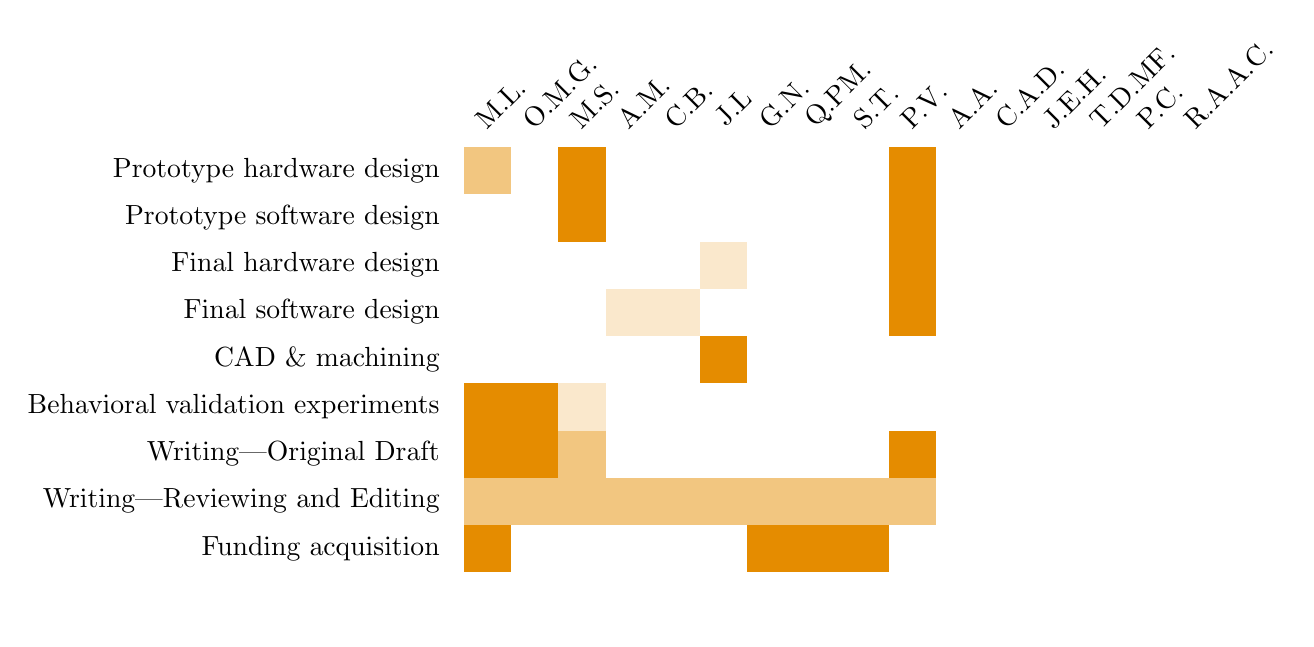
\begin{tikzpicture}[scale=0.6]

    % column labels
    \foreach \a [count=\n] in {
        M.L.,
        O.M.G.,
        M.S.,
        A.M.,
        C.B., 
        J.L,
        G.N.,
        Q.PM.,
        S.T.,
        P.V.,
        A.A.,
        C.A.D.,
        J.E.H.,
        T.D.MF.,
        P.C.,
        R.A.A.C.,
    } {
        \node[col header] at (\n,0) {\a};
    }

    % row labels
    \foreach \a [count=\i] in {
        Prototype hardware design,
        Prototype software design,
        Final hardware design,
        Final software design,
        CAD \& machining,
        Behavioral validation experiments,
        Writing---Original Draft,
        Writing---Reviewing and Editing,
        Funding acquisition,
    } {
        \node[row label] at (0,-\i) {\a};
    }

    \foreach \y [count=\n] in {
        {\mid,0,\hi,0,0,0,0,0,0,\hi},  %hardware prototype
        {0,0,\hi,0,0,0,0,0,0,\hi},     %software prototype
        {0,0,0,0,0,\lo,0,0,0,\hi},     %hardware
        {0,0,0,\lo,\lo,0,0,0,0,\hi},   %software
        {0,0,0,0,0,\hi,0,0,0,0},       %CAD
        {\hi,\hi,\lo,0,0,0,0,0,0,0,0}, % Behav valid
        {\hi,\hi,\mid,0,0,0,0,0,0,\hi}, %Writing: draft
        {\mid,\mid,\mid,\mid,\mid,\mid,\mid,\mid,\mid,\mid}, %Writing: edits
        {\hi,0,0,0,0,0,\hi,\hi,\hi,0},  % Funding
    } {
        % heatmap tiles
        \foreach \x [count=\m] in \y {
            \node[fill=tilecolor!\x!white, tile, text=white] (tile) at (\m,-\n) {};
        }
    }

    % description below heatmap 
    %\node [legend line] at (1, 0 |- tile.south) {*, $^\dagger$ these authors contributed equally};

\end{tikzpicture}